\documentclass[twoside]{book}

% Packages required by doxygen
\usepackage{fixltx2e}
\usepackage{calc}
\usepackage{doxygen}
\usepackage[export]{adjustbox} % also loads graphicx
\usepackage{graphicx}
\usepackage[utf8]{inputenc}
\usepackage{makeidx}
\usepackage{multicol}
\usepackage{multirow}
\PassOptionsToPackage{warn}{textcomp}
\usepackage{textcomp}
\usepackage[nointegrals]{wasysym}
\usepackage[table]{xcolor}

% Font selection
\usepackage[T1]{fontenc}
\usepackage[scaled=.90]{helvet}
\usepackage{courier}
\usepackage{amssymb}
\usepackage{sectsty}
\renewcommand{\familydefault}{\sfdefault}
\allsectionsfont{%
  \fontseries{bc}\selectfont%
  \color{darkgray}%
}
\renewcommand{\DoxyLabelFont}{%
  \fontseries{bc}\selectfont%
  \color{darkgray}%
}
\newcommand{\+}{\discretionary{\mbox{\scriptsize$\hookleftarrow$}}{}{}}

% Page & text layout
\usepackage{geometry}
\geometry{%
  a4paper,%
  top=2.5cm,%
  bottom=2.5cm,%
  left=2.5cm,%
  right=2.5cm%
}
\tolerance=750
\hfuzz=15pt
\hbadness=750
\setlength{\emergencystretch}{15pt}
\setlength{\parindent}{0cm}
\setlength{\parskip}{3ex plus 2ex minus 2ex}
\makeatletter
\renewcommand{\paragraph}{%
  \@startsection{paragraph}{4}{0ex}{-1.0ex}{1.0ex}{%
    \normalfont\normalsize\bfseries\SS@parafont%
  }%
}
\renewcommand{\subparagraph}{%
  \@startsection{subparagraph}{5}{0ex}{-1.0ex}{1.0ex}{%
    \normalfont\normalsize\bfseries\SS@subparafont%
  }%
}
\makeatother

% Headers & footers
\usepackage{fancyhdr}
\pagestyle{fancyplain}
\fancyhead[LE]{\fancyplain{}{\bfseries\thepage}}
\fancyhead[CE]{\fancyplain{}{}}
\fancyhead[RE]{\fancyplain{}{\bfseries\leftmark}}
\fancyhead[LO]{\fancyplain{}{\bfseries\rightmark}}
\fancyhead[CO]{\fancyplain{}{}}
\fancyhead[RO]{\fancyplain{}{\bfseries\thepage}}
\fancyfoot[LE]{\fancyplain{}{}}
\fancyfoot[CE]{\fancyplain{}{}}
\fancyfoot[RE]{\fancyplain{}{\bfseries\scriptsize Generated by Doxygen }}
\fancyfoot[LO]{\fancyplain{}{\bfseries\scriptsize Generated by Doxygen }}
\fancyfoot[CO]{\fancyplain{}{}}
\fancyfoot[RO]{\fancyplain{}{}}
\renewcommand{\footrulewidth}{0.4pt}
\renewcommand{\chaptermark}[1]{%
  \markboth{#1}{}%
}
\renewcommand{\sectionmark}[1]{%
  \markright{\thesection\ #1}%
}

% Indices & bibliography
\usepackage{natbib}
\usepackage[titles]{tocloft}
\setcounter{tocdepth}{3}
\setcounter{secnumdepth}{5}
\makeindex

% Hyperlinks (required, but should be loaded last)
\usepackage{ifpdf}
\ifpdf
  \usepackage[pdftex,pagebackref=true]{hyperref}
\else
  \usepackage[ps2pdf,pagebackref=true]{hyperref}
\fi
\hypersetup{%
  colorlinks=true,%
  linkcolor=blue,%
  citecolor=blue,%
  unicode%
}

% Custom commands
\newcommand{\clearemptydoublepage}{%
  \newpage{\pagestyle{empty}\cleardoublepage}%
}

\usepackage{caption}
\captionsetup{labelsep=space,justification=centering,font={bf},singlelinecheck=off,skip=4pt,position=top}

%===== C O N T E N T S =====

\begin{document}

% Titlepage & ToC
\hypersetup{pageanchor=false,
             bookmarksnumbered=true,
             pdfencoding=unicode
            }
\pagenumbering{alph}
\begin{titlepage}
\vspace*{7cm}
\begin{center}%
{\Large I\+A\+Project }\\
\vspace*{1cm}
{\large Generated by Doxygen 1.8.13}\\
\end{center}
\end{titlepage}
\clearemptydoublepage
\pagenumbering{roman}
\tableofcontents
\clearemptydoublepage
\pagenumbering{arabic}
\hypersetup{pageanchor=true}

%--- Begin generated contents ---
\chapter{Hierarchical Index}
\section{Class Hierarchy}
This inheritance list is sorted roughly, but not completely, alphabetically\+:\begin{DoxyCompactList}
\item \contentsline{section}{ann.\+Activation}{\pageref{interfaceann_1_1_activation}}{}
\begin{DoxyCompactList}
\item \contentsline{section}{ann.\+Linear}{\pageref{classann_1_1_linear}}{}
\item \contentsline{section}{ann.\+Sigmoid}{\pageref{classann_1_1_sigmoid}}{}
\item \contentsline{section}{ann.\+Tanh}{\pageref{classann_1_1_tanh}}{}
\end{DoxyCompactList}
\item \contentsline{section}{ann.\+A\+NN}{\pageref{classann_1_1_a_n_n}}{}
\begin{DoxyCompactList}
\item \contentsline{section}{ann.\+One\+Hidden\+Layer}{\pageref{classann_1_1_one_hidden_layer}}{}
\item \contentsline{section}{ann.\+Single\+Layer}{\pageref{classann_1_1_single_layer}}{}
\end{DoxyCompactList}
\item Iterable\begin{DoxyCompactList}
\item \contentsline{section}{ann.\+Input}{\pageref{classann_1_1_input}}{}
\item \contentsline{section}{ann.\+Output}{\pageref{classann_1_1_output}}{}
\end{DoxyCompactList}
\item \contentsline{section}{ann.\+Neuron}{\pageref{classann_1_1_neuron}}{}
\begin{DoxyCompactList}
\item \contentsline{section}{ann.\+Input\+Neuron}{\pageref{classann_1_1_input_neuron}}{}
\end{DoxyCompactList}
\item Application\begin{DoxyCompactList}
\item \contentsline{section}{ann.\+Mnist\+Data}{\pageref{classann_1_1_mnist_data}}{}
\end{DoxyCompactList}
\end{DoxyCompactList}

\chapter{Class Index}
\section{Class List}
Here are the classes, structs, unions and interfaces with brief descriptions\+:\begin{DoxyCompactList}
\item\contentsline{section}{\hyperlink{interfaceann_1_1_activation}{ann.\+Activation} }{\pageref{interfaceann_1_1_activation}}{}
\item\contentsline{section}{\hyperlink{classann_1_1_a_n_n}{ann.\+A\+NN} }{\pageref{classann_1_1_a_n_n}}{}
\item\contentsline{section}{\hyperlink{classann_1_1_input}{ann.\+Input} }{\pageref{classann_1_1_input}}{}
\item\contentsline{section}{\hyperlink{classann_1_1_input_neuron}{ann.\+Input\+Neuron} }{\pageref{classann_1_1_input_neuron}}{}
\item\contentsline{section}{\hyperlink{classann_1_1_linear}{ann.\+Linear} }{\pageref{classann_1_1_linear}}{}
\item\contentsline{section}{\hyperlink{classann_1_1_mnist_data}{ann.\+Mnist\+Data} }{\pageref{classann_1_1_mnist_data}}{}
\item\contentsline{section}{\hyperlink{classann_1_1_neuron}{ann.\+Neuron} }{\pageref{classann_1_1_neuron}}{}
\item\contentsline{section}{\hyperlink{classann_1_1_one_hidden_layer}{ann.\+One\+Hidden\+Layer} }{\pageref{classann_1_1_one_hidden_layer}}{}
\item\contentsline{section}{\hyperlink{classann_1_1_output}{ann.\+Output} }{\pageref{classann_1_1_output}}{}
\item\contentsline{section}{\hyperlink{classann_1_1_sigmoid}{ann.\+Sigmoid} }{\pageref{classann_1_1_sigmoid}}{}
\item\contentsline{section}{\hyperlink{classann_1_1_single_layer}{ann.\+Single\+Layer} }{\pageref{classann_1_1_single_layer}}{}
\item\contentsline{section}{\hyperlink{classann_1_1_tanh}{ann.\+Tanh} }{\pageref{classann_1_1_tanh}}{}
\end{DoxyCompactList}

\chapter{Class Documentation}
\hypertarget{interfaceann_1_1_activation}{}\section{ann.\+Activation Interface Reference}
\label{interfaceann_1_1_activation}\index{ann.\+Activation@{ann.\+Activation}}
Inheritance diagram for ann.\+Activation\+:\begin{figure}[H]
\begin{center}
\leavevmode
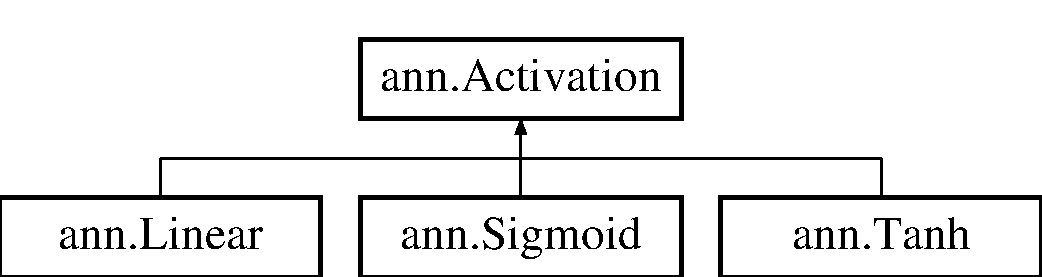
\includegraphics[height=2.000000cm]{interfaceann_1_1_activation}
\end{center}
\end{figure}
\subsection*{Public Member Functions}
\begin{DoxyCompactItemize}
\item 
\mbox{\Hypertarget{interfaceann_1_1_activation_a792856c4231dfcccc7cf7ab9739bc48f}\label{interfaceann_1_1_activation_a792856c4231dfcccc7cf7ab9739bc48f}} 
double {\bfseries activate} (double v)
\end{DoxyCompactItemize}


The documentation for this interface was generated from the following file\+:\begin{DoxyCompactItemize}
\item 
C\+:/\+Users/\+Nick/\+Desktop/\+M1 M\+I\+A\+G\+E/\+Iam\+The\+One/\+Intelligence-\/\+Artificielle/\+Projet/iaproject/src/ann/Activation.\+java\end{DoxyCompactItemize}

\hypertarget{classann_1_1_a_n_n}{}\section{ann.\+A\+NN Class Reference}
\label{classann_1_1_a_n_n}\index{ann.\+A\+NN@{ann.\+A\+NN}}
Inheritance diagram for ann.\+A\+NN\+:\begin{figure}[H]
\begin{center}
\leavevmode
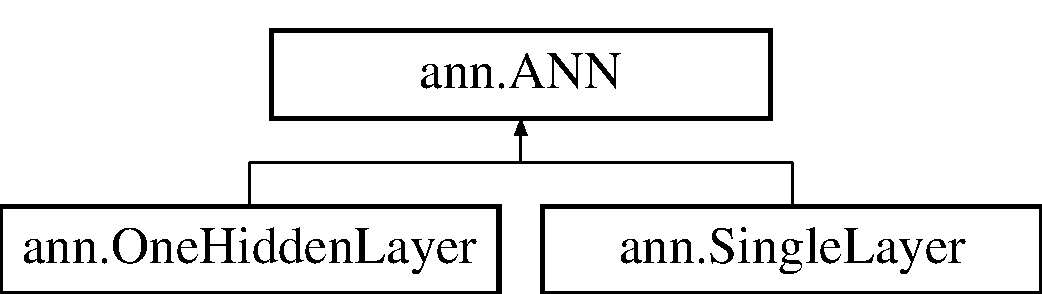
\includegraphics[height=2.000000cm]{classann_1_1_a_n_n}
\end{center}
\end{figure}
\subsection*{Public Member Functions}
\begin{DoxyCompactItemize}
\item 
abstract Map$<$ Integer, Double $>$ \hyperlink{classann_1_1_a_n_n_a9e4c633b9b365c89245bbb441c86d71c}{train} (int num\+Iterations)
\item 
abstract \hyperlink{classann_1_1_output}{Output} \hyperlink{classann_1_1_a_n_n_adc3da5c04b719a2d7c93ef5af2e898b7}{feed} (\hyperlink{classann_1_1_input}{Input} in)
\item 
double \hyperlink{classann_1_1_a_n_n_aa7ab72312b84e639aa84b6fbee5c9df1}{test} (Map$<$ \hyperlink{classann_1_1_input}{Input}, \hyperlink{classann_1_1_output}{Output} $>$ data, int it)
\end{DoxyCompactItemize}


\subsection{Detailed Description}
Abstract class for an artificial neural network \begin{DoxyAuthor}{Author}
stephane 
\end{DoxyAuthor}


\subsection{Member Function Documentation}
\mbox{\Hypertarget{classann_1_1_a_n_n_adc3da5c04b719a2d7c93ef5af2e898b7}\label{classann_1_1_a_n_n_adc3da5c04b719a2d7c93ef5af2e898b7}} 
\index{ann\+::\+A\+NN@{ann\+::\+A\+NN}!feed@{feed}}
\index{feed@{feed}!ann\+::\+A\+NN@{ann\+::\+A\+NN}}
\subsubsection{\texorpdfstring{feed()}{feed()}}
{\footnotesize\ttfamily abstract \hyperlink{classann_1_1_output}{Output} ann.\+A\+N\+N.\+feed (\begin{DoxyParamCaption}\item[{\hyperlink{classann_1_1_input}{Input}}]{in }\end{DoxyParamCaption})\hspace{0.3cm}{\ttfamily [abstract]}}

Methods that computes the output of the neural network given the input 
\begin{DoxyParams}{Parameters}
{\em in} & input data of the neural network \\
\hline
\end{DoxyParams}
\begin{DoxyReturn}{Returns}
the output of the neural network (it is stored in an object output that contains a vector of the values of each neurons in the output layer 
\end{DoxyReturn}
\mbox{\Hypertarget{classann_1_1_a_n_n_aa7ab72312b84e639aa84b6fbee5c9df1}\label{classann_1_1_a_n_n_aa7ab72312b84e639aa84b6fbee5c9df1}} 
\index{ann\+::\+A\+NN@{ann\+::\+A\+NN}!test@{test}}
\index{test@{test}!ann\+::\+A\+NN@{ann\+::\+A\+NN}}
\subsubsection{\texorpdfstring{test()}{test()}}
{\footnotesize\ttfamily double ann.\+A\+N\+N.\+test (\begin{DoxyParamCaption}\item[{Map$<$ \hyperlink{classann_1_1_input}{Input}, \hyperlink{classann_1_1_output}{Output} $>$}]{data,  }\item[{int}]{it }\end{DoxyParamCaption})}

Methods that computes the number of mistakes of the neural network on the testing data\+: for each example in the training data, the method compares the output of the network with the label of the data and counts the number of mistakes. 
\begin{DoxyParams}{Parameters}
{\em data} & map that contains a set of data (usually used with the testing data) \\
\hline
{\em it} & the number of iterations when this test is called (it is only used to print the result on the console) \\
\hline
\end{DoxyParams}
\begin{DoxyReturn}{Returns}
the number of mistakes made on the data set. 
\end{DoxyReturn}
\mbox{\Hypertarget{classann_1_1_a_n_n_a9e4c633b9b365c89245bbb441c86d71c}\label{classann_1_1_a_n_n_a9e4c633b9b365c89245bbb441c86d71c}} 
\index{ann\+::\+A\+NN@{ann\+::\+A\+NN}!train@{train}}
\index{train@{train}!ann\+::\+A\+NN@{ann\+::\+A\+NN}}
\subsubsection{\texorpdfstring{train()}{train()}}
{\footnotesize\ttfamily abstract Map$<$Integer,Double$>$ ann.\+A\+N\+N.\+train (\begin{DoxyParamCaption}\item[{int}]{num\+Iterations }\end{DoxyParamCaption})\hspace{0.3cm}{\ttfamily [abstract]}}

method that trains the neural network for a certain number of iterations (no convergence test is used). 
\begin{DoxyParams}{Parameters}
{\em num\+Iterations} & is the number of iterations, i.\+e. the number of times the algorithm will update using the entire training data \\
\hline
\end{DoxyParams}
\begin{DoxyReturn}{Returns}
returns the dynamics of the error\+: it contains a map that associate one iteration number and the number of mistakes done on the testing set. 
\end{DoxyReturn}


The documentation for this class was generated from the following file\+:\begin{DoxyCompactItemize}
\item 
C\+:/\+Users/\+Nick/\+Desktop/\+M1 M\+I\+A\+G\+E/\+Iam\+The\+One/\+Intelligence-\/\+Artificielle/\+Projet/iaproject/src/ann/A\+N\+N.\+java\end{DoxyCompactItemize}

\hypertarget{classann_1_1_input}{}\section{ann.\+Input Class Reference}
\label{classann_1_1_input}\index{ann.\+Input@{ann.\+Input}}
Inheritance diagram for ann.\+Input\+:\begin{figure}[H]
\begin{center}
\leavevmode
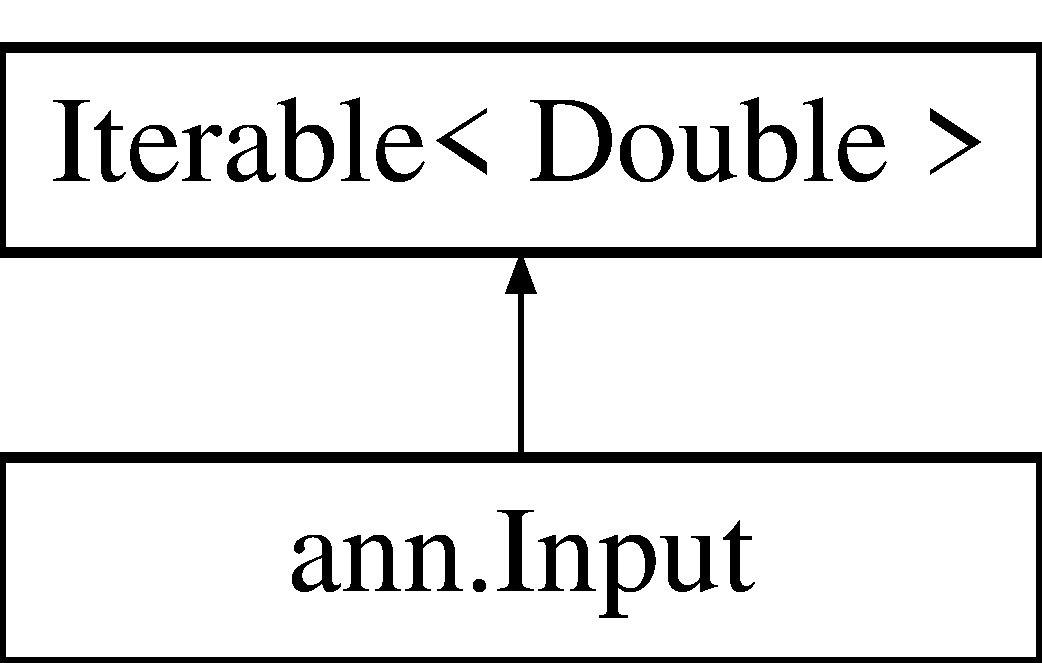
\includegraphics[height=2.000000cm]{classann_1_1_input}
\end{center}
\end{figure}
\subsection*{Public Member Functions}
\begin{DoxyCompactItemize}
\item 
\mbox{\Hypertarget{classann_1_1_input_a58e4d4bd454620c64b162792f05398a8}\label{classann_1_1_input_a58e4d4bd454620c64b162792f05398a8}} 
{\bfseries Input} (int size)
\item 
\mbox{\Hypertarget{classann_1_1_input_a56db4af5fd8a2888e14cf6610b1b9067}\label{classann_1_1_input_a56db4af5fd8a2888e14cf6610b1b9067}} 
{\bfseries Input} (int num\+Rows, int num\+Cols)
\item 
\mbox{\Hypertarget{classann_1_1_input_ac57941ba7f3a4562e90d4a686e274cb6}\label{classann_1_1_input_ac57941ba7f3a4562e90d4a686e274cb6}} 
void {\bfseries set\+Value} (int row, int col, int val)
\item 
\mbox{\Hypertarget{classann_1_1_input_a997d6cbb6b015e32b884f1763c3709c2}\label{classann_1_1_input_a997d6cbb6b015e32b884f1763c3709c2}} 
double {\bfseries get\+Value} (int row, int col)
\item 
\mbox{\Hypertarget{classann_1_1_input_a10cf38f57f0f5351e99c3ad997035b4c}\label{classann_1_1_input_a10cf38f57f0f5351e99c3ad997035b4c}} 
String {\bfseries to\+String} ()
\item 
\mbox{\Hypertarget{classann_1_1_input_abde8c7c03ebcaceebc918afb3d3a49e1}\label{classann_1_1_input_abde8c7c03ebcaceebc918afb3d3a49e1}} 
Iterator$<$ Double $>$ {\bfseries iterator} ()
\end{DoxyCompactItemize}


The documentation for this class was generated from the following file\+:\begin{DoxyCompactItemize}
\item 
C\+:/\+Users/\+Nick/\+Desktop/\+M1 M\+I\+A\+G\+E/\+Iam\+The\+One/\+Intelligence-\/\+Artificielle/\+Projet/src/ann/Input.\+java\end{DoxyCompactItemize}

\hypertarget{classann_1_1_input_neuron}{}\section{ann.\+Input\+Neuron Class Reference}
\label{classann_1_1_input_neuron}\index{ann.\+Input\+Neuron@{ann.\+Input\+Neuron}}
Inheritance diagram for ann.\+Input\+Neuron\+:\begin{figure}[H]
\begin{center}
\leavevmode
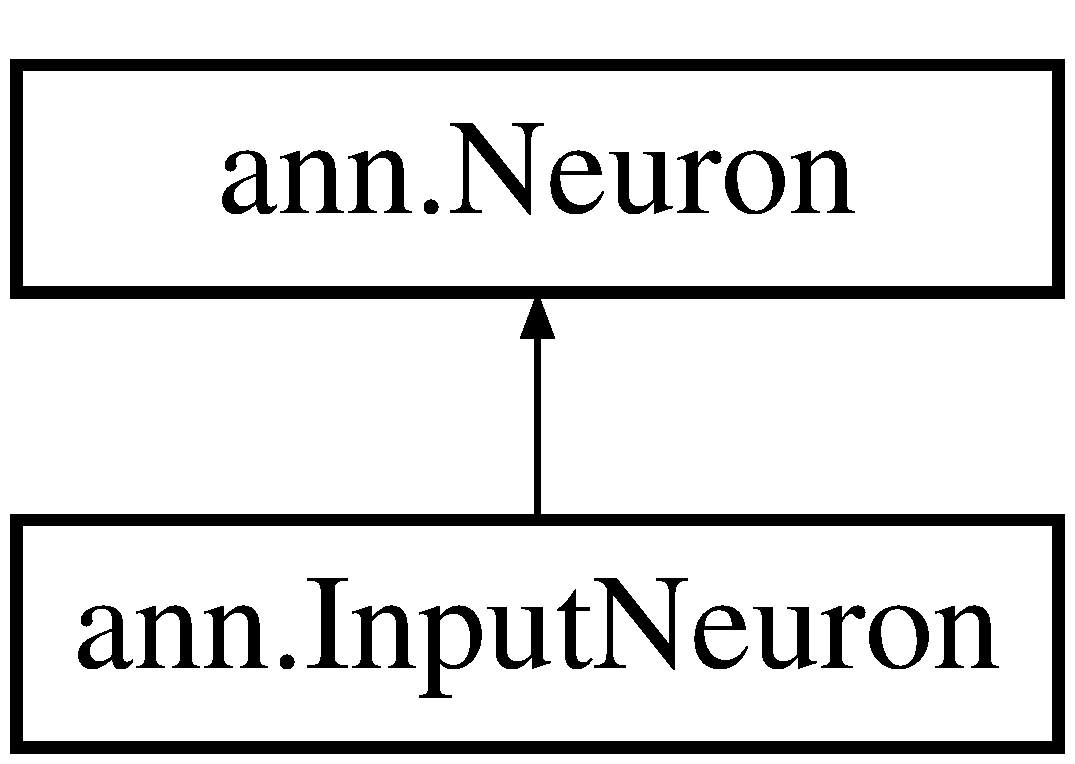
\includegraphics[height=2.000000cm]{classann_1_1_input_neuron}
\end{center}
\end{figure}
\subsection*{Public Member Functions}
\begin{DoxyCompactItemize}
\item 
\mbox{\Hypertarget{classann_1_1_input_neuron_aff4d145c16f3c5e6b667a739465a3866}\label{classann_1_1_input_neuron_aff4d145c16f3c5e6b667a739465a3866}} 
{\bfseries Input\+Neuron} (double normalise)
\item 
\mbox{\Hypertarget{classann_1_1_input_neuron_a6a02b1d84db4ae32922ae59707a0c039}\label{classann_1_1_input_neuron_a6a02b1d84db4ae32922ae59707a0c039}} 
void {\bfseries feed} (double val)
\end{DoxyCompactItemize}
\subsection*{Additional Inherited Members}


\subsection{Detailed Description}
Models a neuron in the input layer. This neuron does not learn anything (there are no weights!) it is simply used to feed the data in the network. \begin{DoxyAuthor}{Author}
stephane 
\end{DoxyAuthor}


The documentation for this class was generated from the following file\+:\begin{DoxyCompactItemize}
\item 
C\+:/\+Users/\+Nick/\+Desktop/\+M1 M\+I\+A\+G\+E/\+Iam\+The\+One/\+Intelligence-\/\+Artificielle/\+Projet/src/ann/Input\+Neuron.\+java\end{DoxyCompactItemize}

\hypertarget{classann_1_1_linear}{}\section{ann.\+Linear Class Reference}
\label{classann_1_1_linear}\index{ann.\+Linear@{ann.\+Linear}}
Inheritance diagram for ann.\+Linear\+:\begin{figure}[H]
\begin{center}
\leavevmode
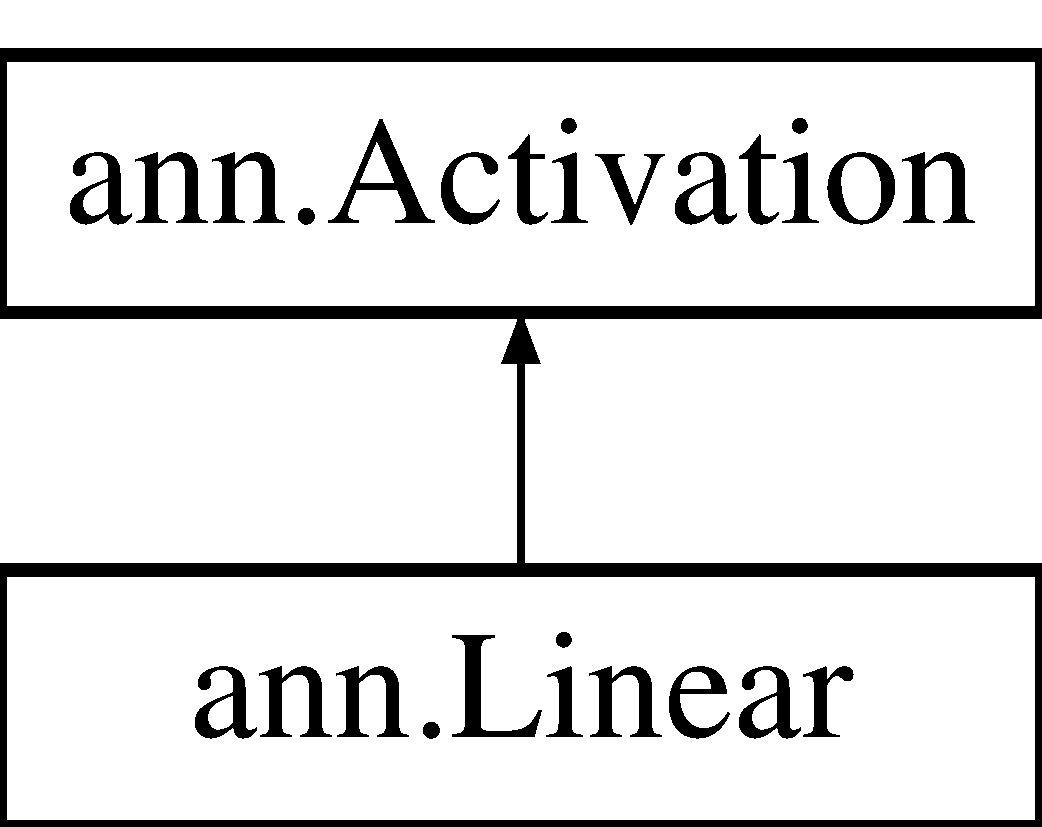
\includegraphics[height=2.000000cm]{classann_1_1_linear}
\end{center}
\end{figure}
\subsection*{Public Member Functions}
\begin{DoxyCompactItemize}
\item 
\mbox{\Hypertarget{classann_1_1_linear_ae68f09cd9d9fc93ac9c00f61730b82fb}\label{classann_1_1_linear_ae68f09cd9d9fc93ac9c00f61730b82fb}} 
double {\bfseries activate} (double val)
\end{DoxyCompactItemize}


The documentation for this class was generated from the following file\+:\begin{DoxyCompactItemize}
\item 
C\+:/\+Users/\+Nick/\+Desktop/\+M1 M\+I\+A\+G\+E/\+Iam\+The\+One/\+Intelligence-\/\+Artificielle/\+Projet/src/ann/Linear.\+java\end{DoxyCompactItemize}

\hypertarget{classann_1_1_mnist_data}{}\section{ann.\+Mnist\+Data Class Reference}
\label{classann_1_1_mnist_data}\index{ann.\+Mnist\+Data@{ann.\+Mnist\+Data}}
Inheritance diagram for ann.\+Mnist\+Data\+:\begin{figure}[H]
\begin{center}
\leavevmode
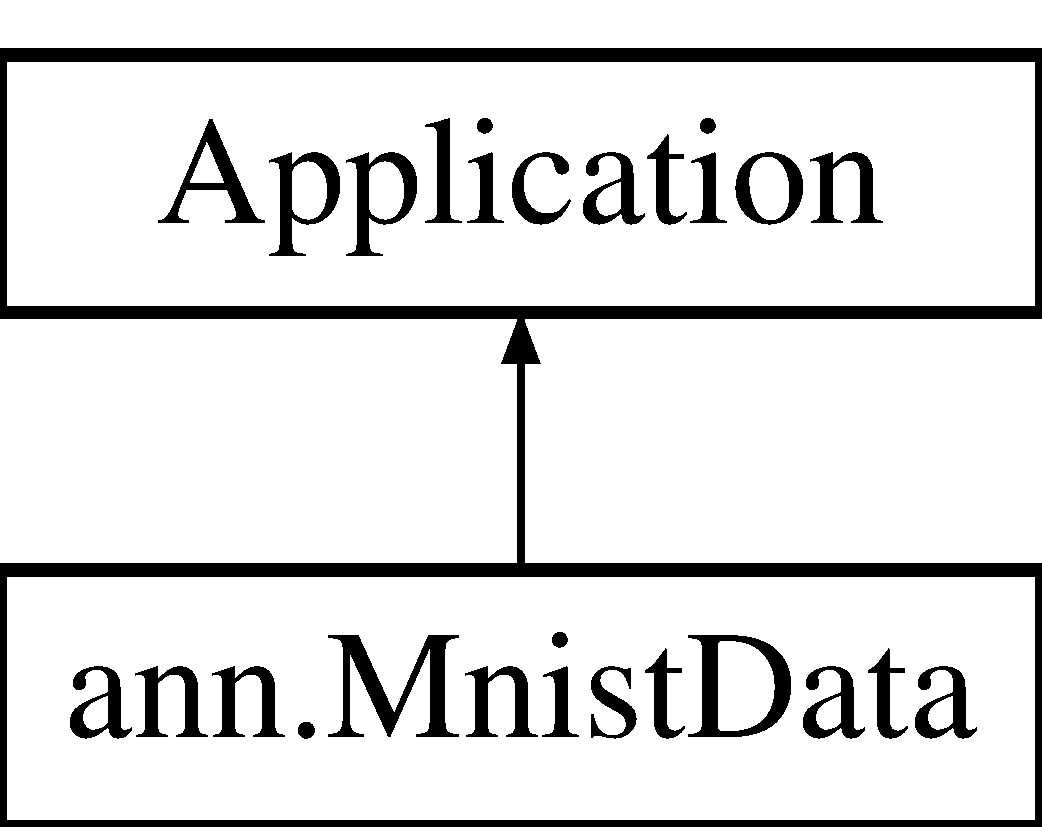
\includegraphics[height=2.000000cm]{classann_1_1_mnist_data}
\end{center}
\end{figure}
\subsection*{Public Member Functions}
\begin{DoxyCompactItemize}
\item 
void \hyperlink{classann_1_1_mnist_data_a163423e53cf98cbc9c7517f40a1a2476}{start} (Stage primary\+Stage)  throws Exception 
\end{DoxyCompactItemize}
\subsection*{Static Public Member Functions}
\begin{DoxyCompactItemize}
\item 
static Map$<$ \hyperlink{classann_1_1_input}{Input}, \hyperlink{classann_1_1_output}{Output} $>$ \hyperlink{classann_1_1_mnist_data_af92e544d110867d6a1324bfb9ec6b3f2}{read\+Data} (String data\+File\+Path, String label\+File\+Path)  throws I\+O\+Exception 
\item 
static void \hyperlink{classann_1_1_mnist_data_a927889494e75519b70b5364b391cb37d}{main} (String\mbox{[}$\,$\mbox{]} args)
\end{DoxyCompactItemize}


\subsection{Detailed Description}
Class that reads the M\+N\+I\+ST data and run simulation from a user interface

\begin{DoxyAuthor}{Author}
stephane 
\end{DoxyAuthor}


\subsection{Member Function Documentation}
\mbox{\Hypertarget{classann_1_1_mnist_data_a927889494e75519b70b5364b391cb37d}\label{classann_1_1_mnist_data_a927889494e75519b70b5364b391cb37d}} 
\index{ann\+::\+Mnist\+Data@{ann\+::\+Mnist\+Data}!main@{main}}
\index{main@{main}!ann\+::\+Mnist\+Data@{ann\+::\+Mnist\+Data}}
\subsubsection{\texorpdfstring{main()}{main()}}
{\footnotesize\ttfamily static void ann.\+Mnist\+Data.\+main (\begin{DoxyParamCaption}\item[{String \mbox{[}$\,$\mbox{]}}]{args }\end{DoxyParamCaption})\hspace{0.3cm}{\ttfamily [static]}}

launch the simulator\+: when ran with no argument, the program simply trains a single layer neural network and stops; ran with any argument, it lauches a user interface.


\begin{DoxyParams}{Parameters}
{\em args} & \\
\hline
\end{DoxyParams}
\mbox{\Hypertarget{classann_1_1_mnist_data_af92e544d110867d6a1324bfb9ec6b3f2}\label{classann_1_1_mnist_data_af92e544d110867d6a1324bfb9ec6b3f2}} 
\index{ann\+::\+Mnist\+Data@{ann\+::\+Mnist\+Data}!read\+Data@{read\+Data}}
\index{read\+Data@{read\+Data}!ann\+::\+Mnist\+Data@{ann\+::\+Mnist\+Data}}
\subsubsection{\texorpdfstring{read\+Data()}{readData()}}
{\footnotesize\ttfamily static Map$<$\hyperlink{classann_1_1_input}{Input},\hyperlink{classann_1_1_output}{Output}$>$ ann.\+Mnist\+Data.\+read\+Data (\begin{DoxyParamCaption}\item[{String}]{data\+File\+Path,  }\item[{String}]{label\+File\+Path }\end{DoxyParamCaption}) throws I\+O\+Exception\hspace{0.3cm}{\ttfamily [static]}}

Read two data files from the M\+N\+I\+ST repository\+: one file contains the training instances, the other the label of the training instances


\begin{DoxyParams}{Parameters}
{\em data\+File\+Path} & path of the data file containing the training data \\
\hline
{\em label\+File\+Path} & label name of the data file containing the label of the training data \\
\hline
\end{DoxyParams}
\begin{DoxyReturn}{Returns}
a map that associates to each data its associated label 
\end{DoxyReturn}

\begin{DoxyExceptions}{Exceptions}
{\em I\+O\+Exception} & \\
\hline
\end{DoxyExceptions}
\mbox{\Hypertarget{classann_1_1_mnist_data_a163423e53cf98cbc9c7517f40a1a2476}\label{classann_1_1_mnist_data_a163423e53cf98cbc9c7517f40a1a2476}} 
\index{ann\+::\+Mnist\+Data@{ann\+::\+Mnist\+Data}!start@{start}}
\index{start@{start}!ann\+::\+Mnist\+Data@{ann\+::\+Mnist\+Data}}
\subsubsection{\texorpdfstring{start()}{start()}}
{\footnotesize\ttfamily void ann.\+Mnist\+Data.\+start (\begin{DoxyParamCaption}\item[{Stage}]{primary\+Stage }\end{DoxyParamCaption}) throws Exception}

Method that controls the user interface. 

The documentation for this class was generated from the following file\+:\begin{DoxyCompactItemize}
\item 
C\+:/\+Users/\+Nick/\+Desktop/\+M1 M\+I\+A\+G\+E/\+Iam\+The\+One/\+Intelligence-\/\+Artificielle/\+Projet/src/ann/Mnist\+Data.\+java\end{DoxyCompactItemize}

\hypertarget{classann_1_1_neuron}{}\section{ann.\+Neuron Class Reference}
\label{classann_1_1_neuron}\index{ann.\+Neuron@{ann.\+Neuron}}
Inheritance diagram for ann.\+Neuron\+:\begin{figure}[H]
\begin{center}
\leavevmode
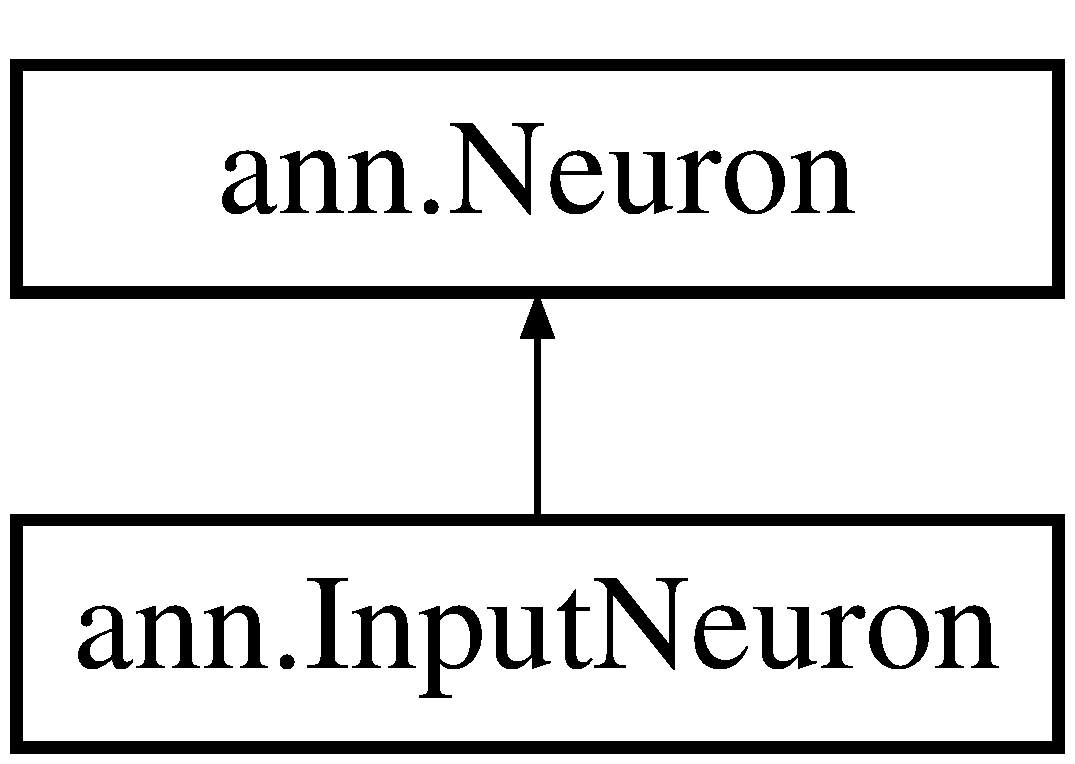
\includegraphics[height=2.000000cm]{classann_1_1_neuron}
\end{center}
\end{figure}
\subsection*{Public Member Functions}
\begin{DoxyCompactItemize}
\item 
double \hyperlink{classann_1_1_neuron_adaea18e61d0a87b9e47cc41c552417dd}{get\+Error} ()
\item 
\hyperlink{classann_1_1_neuron_ab0f583ed1a1c83ed5ff5bc24c77db902}{Neuron} (\hyperlink{interfaceann_1_1_activation}{Activation} h)
\item 
\mbox{\Hypertarget{classann_1_1_neuron_a0ba98646afe2473db08616ceffe80551}\label{classann_1_1_neuron_a0ba98646afe2473db08616ceffe80551}} 
void {\bfseries add\+Parent} (\hyperlink{classann_1_1_neuron}{Neuron} parent)
\item 
\mbox{\Hypertarget{classann_1_1_neuron_a84df35de6af704840e26dd618ea62cdf}\label{classann_1_1_neuron_a84df35de6af704840e26dd618ea62cdf}} 
void {\bfseries add\+Child} (\hyperlink{classann_1_1_neuron}{Neuron} child)
\item 
void \hyperlink{classann_1_1_neuron_aa1544b3c4a7e5a002eef88277126d4f5}{init\+Weights} ()
\item 
void \hyperlink{classann_1_1_neuron_aaae37fc2d90b1f42b4fd4ba00e23dc04}{feed} ()
\item 
void \hyperlink{classann_1_1_neuron_acb5bda80a06130b2c68bba370ee27a84}{back\+Propagate} (double target)
\item 
double \hyperlink{classann_1_1_neuron_ae8c43d9defae7bb44d8562382474f87c}{get\+Current\+Output} ()
\item 
String \hyperlink{classann_1_1_neuron_a22d903dc7a9e7693b77c3b407359a78a}{to\+String} ()
\end{DoxyCompactItemize}
\subsection*{Static Public Attributes}
\begin{DoxyCompactItemize}
\item 
static Random \hyperlink{classann_1_1_neuron_ac7d2bce61156cee5b79e960bf719ee6b}{generator}
\end{DoxyCompactItemize}
\subsection*{Protected Attributes}
\begin{DoxyCompactItemize}
\item 
double \hyperlink{classann_1_1_neuron_a50568ffff3bd8194ded913041414b244}{out}
\item 
double \hyperlink{classann_1_1_neuron_a68c3c65ea538d533aae8a343b043d921}{error}
\end{DoxyCompactItemize}


\subsection{Constructor \& Destructor Documentation}
\mbox{\Hypertarget{classann_1_1_neuron_ab0f583ed1a1c83ed5ff5bc24c77db902}\label{classann_1_1_neuron_ab0f583ed1a1c83ed5ff5bc24c77db902}} 
\index{ann\+::\+Neuron@{ann\+::\+Neuron}!Neuron@{Neuron}}
\index{Neuron@{Neuron}!ann\+::\+Neuron@{ann\+::\+Neuron}}
\subsubsection{\texorpdfstring{Neuron()}{Neuron()}}
{\footnotesize\ttfamily ann.\+Neuron.\+Neuron (\begin{DoxyParamCaption}\item[{\hyperlink{interfaceann_1_1_activation}{Activation}}]{h }\end{DoxyParamCaption})}

Constructor 
\begin{DoxyParams}{Parameters}
{\em h} & is an activation function (linear, sigmoid, tanh) \\
\hline
\end{DoxyParams}


\subsection{Member Function Documentation}
\mbox{\Hypertarget{classann_1_1_neuron_acb5bda80a06130b2c68bba370ee27a84}\label{classann_1_1_neuron_acb5bda80a06130b2c68bba370ee27a84}} 
\index{ann\+::\+Neuron@{ann\+::\+Neuron}!back\+Propagate@{back\+Propagate}}
\index{back\+Propagate@{back\+Propagate}!ann\+::\+Neuron@{ann\+::\+Neuron}}
\subsubsection{\texorpdfstring{back\+Propagate()}{backPropagate()}}
{\footnotesize\ttfamily void ann.\+Neuron.\+back\+Propagate (\begin{DoxyParamCaption}\item[{double}]{target }\end{DoxyParamCaption})}

back propagation for a neuron in the output layer 
\begin{DoxyParams}{Parameters}
{\em val} & is the correct value. \\
\hline
\end{DoxyParams}
\mbox{\Hypertarget{classann_1_1_neuron_aaae37fc2d90b1f42b4fd4ba00e23dc04}\label{classann_1_1_neuron_aaae37fc2d90b1f42b4fd4ba00e23dc04}} 
\index{ann\+::\+Neuron@{ann\+::\+Neuron}!feed@{feed}}
\index{feed@{feed}!ann\+::\+Neuron@{ann\+::\+Neuron}}
\subsubsection{\texorpdfstring{feed()}{feed()}}
{\footnotesize\ttfamily void ann.\+Neuron.\+feed (\begin{DoxyParamCaption}{ }\end{DoxyParamCaption})}

Computes the output of a neuron that is either in the hidden layer or in the output layer. (there are no arguments as the neuron is not an input\+Neuron) \mbox{\Hypertarget{classann_1_1_neuron_ae8c43d9defae7bb44d8562382474f87c}\label{classann_1_1_neuron_ae8c43d9defae7bb44d8562382474f87c}} 
\index{ann\+::\+Neuron@{ann\+::\+Neuron}!get\+Current\+Output@{get\+Current\+Output}}
\index{get\+Current\+Output@{get\+Current\+Output}!ann\+::\+Neuron@{ann\+::\+Neuron}}
\subsubsection{\texorpdfstring{get\+Current\+Output()}{getCurrentOutput()}}
{\footnotesize\ttfamily double ann.\+Neuron.\+get\+Current\+Output (\begin{DoxyParamCaption}{ }\end{DoxyParamCaption})}

returns the current ouput (it should be called once the output has been computed, i.\+e. after calling feed) \begin{DoxyReturn}{Returns}
the current value of the ouput 
\end{DoxyReturn}
\mbox{\Hypertarget{classann_1_1_neuron_adaea18e61d0a87b9e47cc41c552417dd}\label{classann_1_1_neuron_adaea18e61d0a87b9e47cc41c552417dd}} 
\index{ann\+::\+Neuron@{ann\+::\+Neuron}!get\+Error@{get\+Error}}
\index{get\+Error@{get\+Error}!ann\+::\+Neuron@{ann\+::\+Neuron}}
\subsubsection{\texorpdfstring{get\+Error()}{getError()}}
{\footnotesize\ttfamily double ann.\+Neuron.\+get\+Error (\begin{DoxyParamCaption}{ }\end{DoxyParamCaption})}

returns the current value of the error for that neuron. \begin{DoxyReturn}{Returns}

\end{DoxyReturn}
\mbox{\Hypertarget{classann_1_1_neuron_aa1544b3c4a7e5a002eef88277126d4f5}\label{classann_1_1_neuron_aa1544b3c4a7e5a002eef88277126d4f5}} 
\index{ann\+::\+Neuron@{ann\+::\+Neuron}!init\+Weights@{init\+Weights}}
\index{init\+Weights@{init\+Weights}!ann\+::\+Neuron@{ann\+::\+Neuron}}
\subsubsection{\texorpdfstring{init\+Weights()}{initWeights()}}
{\footnotesize\ttfamily void ann.\+Neuron.\+init\+Weights (\begin{DoxyParamCaption}{ }\end{DoxyParamCaption})}

Initializes randomly the weights of the incoming edges \mbox{\Hypertarget{classann_1_1_neuron_a22d903dc7a9e7693b77c3b407359a78a}\label{classann_1_1_neuron_a22d903dc7a9e7693b77c3b407359a78a}} 
\index{ann\+::\+Neuron@{ann\+::\+Neuron}!to\+String@{to\+String}}
\index{to\+String@{to\+String}!ann\+::\+Neuron@{ann\+::\+Neuron}}
\subsubsection{\texorpdfstring{to\+String()}{toString()}}
{\footnotesize\ttfamily String ann.\+Neuron.\+to\+String (\begin{DoxyParamCaption}{ }\end{DoxyParamCaption})}

returns the name of the neuron $\ast$ 

\subsection{Member Data Documentation}
\mbox{\Hypertarget{classann_1_1_neuron_a68c3c65ea538d533aae8a343b043d921}\label{classann_1_1_neuron_a68c3c65ea538d533aae8a343b043d921}} 
\index{ann\+::\+Neuron@{ann\+::\+Neuron}!error@{error}}
\index{error@{error}!ann\+::\+Neuron@{ann\+::\+Neuron}}
\subsubsection{\texorpdfstring{error}{error}}
{\footnotesize\ttfamily double ann.\+Neuron.\+error\hspace{0.3cm}{\ttfamily [protected]}}

current value of the error of the neuron \mbox{\Hypertarget{classann_1_1_neuron_ac7d2bce61156cee5b79e960bf719ee6b}\label{classann_1_1_neuron_ac7d2bce61156cee5b79e960bf719ee6b}} 
\index{ann\+::\+Neuron@{ann\+::\+Neuron}!generator@{generator}}
\index{generator@{generator}!ann\+::\+Neuron@{ann\+::\+Neuron}}
\subsubsection{\texorpdfstring{generator}{generator}}
{\footnotesize\ttfamily Random ann.\+Neuron.\+generator\hspace{0.3cm}{\ttfamily [static]}}

random number generator \mbox{\Hypertarget{classann_1_1_neuron_a50568ffff3bd8194ded913041414b244}\label{classann_1_1_neuron_a50568ffff3bd8194ded913041414b244}} 
\index{ann\+::\+Neuron@{ann\+::\+Neuron}!out@{out}}
\index{out@{out}!ann\+::\+Neuron@{ann\+::\+Neuron}}
\subsubsection{\texorpdfstring{out}{out}}
{\footnotesize\ttfamily double ann.\+Neuron.\+out\hspace{0.3cm}{\ttfamily [protected]}}

current value of the output of the neuron 

The documentation for this class was generated from the following file\+:\begin{DoxyCompactItemize}
\item 
C\+:/\+Users/\+Nick/\+Desktop/\+M1 M\+I\+A\+G\+E/\+Iam\+The\+One/\+Intelligence-\/\+Artificielle/\+Projet/src/ann/Neuron.\+java\end{DoxyCompactItemize}

\hypertarget{classann_1_1_one_hidden_layer}{}\section{ann.\+One\+Hidden\+Layer Class Reference}
\label{classann_1_1_one_hidden_layer}\index{ann.\+One\+Hidden\+Layer@{ann.\+One\+Hidden\+Layer}}
Inheritance diagram for ann.\+One\+Hidden\+Layer\+:\begin{figure}[H]
\begin{center}
\leavevmode
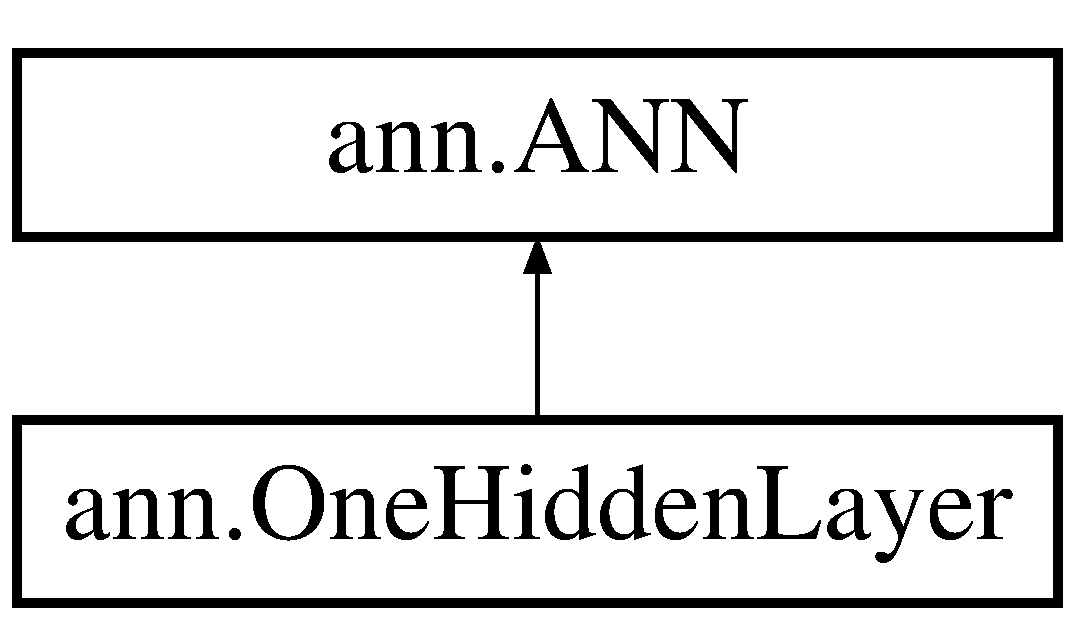
\includegraphics[height=2.000000cm]{classann_1_1_one_hidden_layer}
\end{center}
\end{figure}
\subsection*{Public Member Functions}
\begin{DoxyCompactItemize}
\item 
\mbox{\Hypertarget{classann_1_1_one_hidden_layer_a71b47ecdc9b1847d4758cf6614b4a3b0}\label{classann_1_1_one_hidden_layer_a71b47ecdc9b1847d4758cf6614b4a3b0}} 
{\bfseries One\+Hidden\+Layer} (Map$<$ \hyperlink{classann_1_1_input}{Input}, \hyperlink{classann_1_1_output}{Output} $>$ training\+Data, Map$<$ \hyperlink{classann_1_1_input}{Input}, \hyperlink{classann_1_1_output}{Output} $>$ testing\+Data)
\item 
\mbox{\Hypertarget{classann_1_1_one_hidden_layer_a319db2404483dd4158a7e9266b68f4a4}\label{classann_1_1_one_hidden_layer_a319db2404483dd4158a7e9266b68f4a4}} 
\hyperlink{classann_1_1_output}{Output} {\bfseries feed} (\hyperlink{classann_1_1_input}{Input} in)
\item 
\mbox{\Hypertarget{classann_1_1_one_hidden_layer_a054c8821610b8637e8fa3fa319df2d41}\label{classann_1_1_one_hidden_layer_a054c8821610b8637e8fa3fa319df2d41}} 
Map$<$ Integer, Double $>$ {\bfseries train} (int nb\+Iterations)
\end{DoxyCompactItemize}


The documentation for this class was generated from the following file\+:\begin{DoxyCompactItemize}
\item 
C\+:/\+Users/\+Nick/\+Desktop/\+M1 M\+I\+A\+G\+E/\+Iam\+The\+One/\+Intelligence-\/\+Artificielle/\+Projet/src/ann/One\+Hidden\+Layer.\+java\end{DoxyCompactItemize}

\hypertarget{classann_1_1_output}{}\section{ann.\+Output Class Reference}
\label{classann_1_1_output}\index{ann.\+Output@{ann.\+Output}}
Inheritance diagram for ann.\+Output\+:\begin{figure}[H]
\begin{center}
\leavevmode
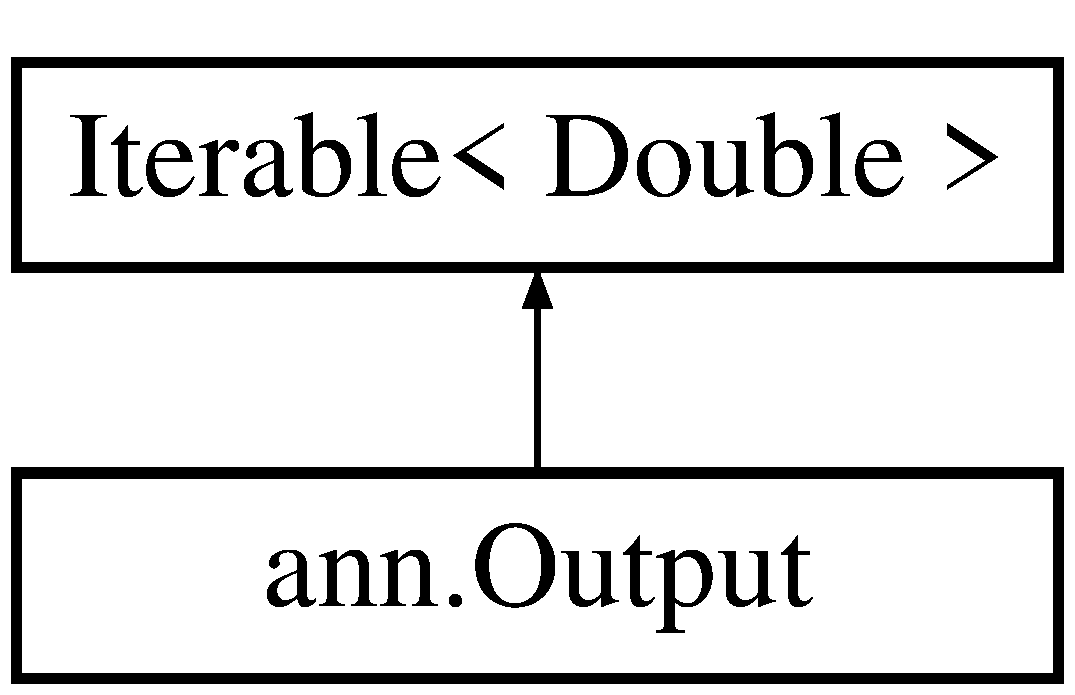
\includegraphics[height=2.000000cm]{classann_1_1_output}
\end{center}
\end{figure}
\subsection*{Public Member Functions}
\begin{DoxyCompactItemize}
\item 
\mbox{\Hypertarget{classann_1_1_output_a7ab3d7c14034fdbe2d6482935f44c9a0}\label{classann_1_1_output_a7ab3d7c14034fdbe2d6482935f44c9a0}} 
{\bfseries Output} (int val)
\item 
\mbox{\Hypertarget{classann_1_1_output_a82f2133f54dcc48c400f894a62eec8f0}\label{classann_1_1_output_a82f2133f54dcc48c400f894a62eec8f0}} 
{\bfseries Output} (double\mbox{[}$\,$\mbox{]} val)
\item 
\mbox{\Hypertarget{classann_1_1_output_a29ceaac61553a61df12b616d3d62ee84}\label{classann_1_1_output_a29ceaac61553a61df12b616d3d62ee84}} 
double \mbox{[}$\,$\mbox{]} {\bfseries get\+Val} ()
\item 
\mbox{\Hypertarget{classann_1_1_output_aa144e935bfe1b126ba527151b1653b69}\label{classann_1_1_output_aa144e935bfe1b126ba527151b1653b69}} 
boolean {\bfseries equals} (Object obj)
\item 
\mbox{\Hypertarget{classann_1_1_output_a7617bd1ab1914c05d797e8bf93b9dcd7}\label{classann_1_1_output_a7617bd1ab1914c05d797e8bf93b9dcd7}} 
String {\bfseries to\+String} ()
\item 
\mbox{\Hypertarget{classann_1_1_output_abf286f373059401bfa29bafbe134ebbc}\label{classann_1_1_output_abf286f373059401bfa29bafbe134ebbc}} 
Iterator$<$ Double $>$ {\bfseries iterator} ()
\end{DoxyCompactItemize}


The documentation for this class was generated from the following file\+:\begin{DoxyCompactItemize}
\item 
C\+:/\+Users/\+Nick/\+Desktop/\+M1 M\+I\+A\+G\+E/\+Iam\+The\+One/\+Intelligence-\/\+Artificielle/\+Projet/src/ann/Output.\+java\end{DoxyCompactItemize}

\hypertarget{classann_1_1_sigmoid}{}\section{ann.\+Sigmoid Class Reference}
\label{classann_1_1_sigmoid}\index{ann.\+Sigmoid@{ann.\+Sigmoid}}
Inheritance diagram for ann.\+Sigmoid\+:\begin{figure}[H]
\begin{center}
\leavevmode
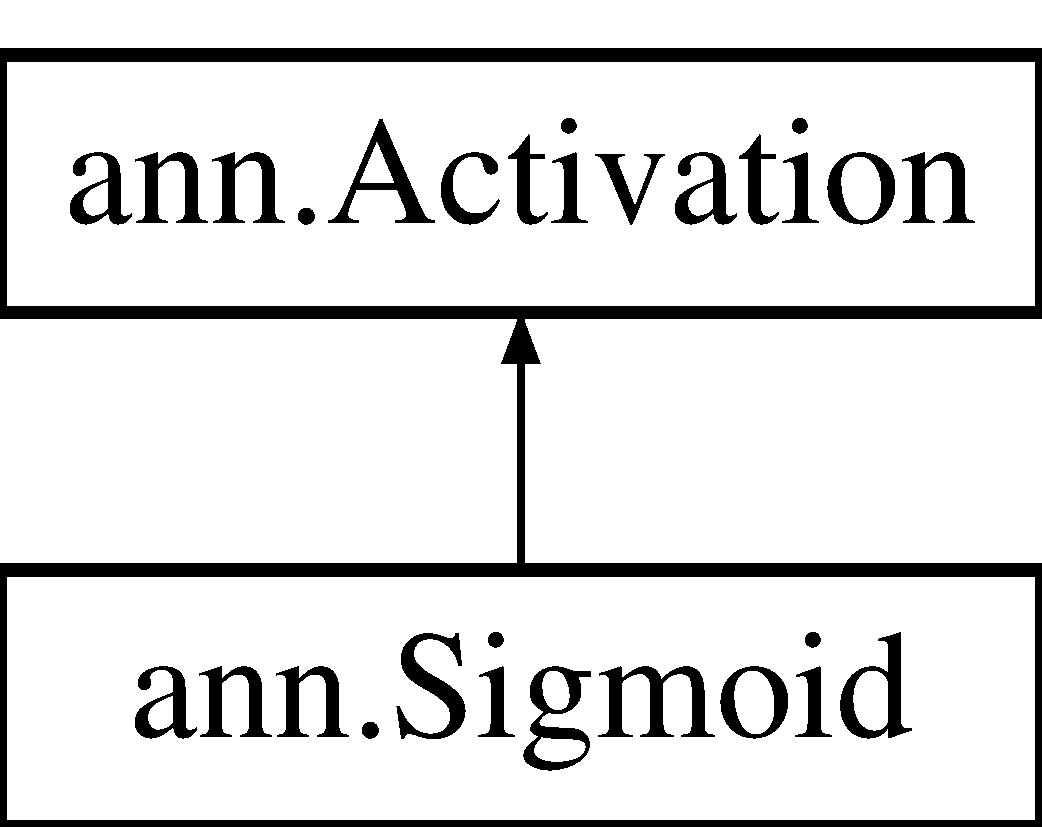
\includegraphics[height=2.000000cm]{classann_1_1_sigmoid}
\end{center}
\end{figure}
\subsection*{Public Member Functions}
\begin{DoxyCompactItemize}
\item 
\mbox{\Hypertarget{classann_1_1_sigmoid_a494474439cd325dce73298bebf90d196}\label{classann_1_1_sigmoid_a494474439cd325dce73298bebf90d196}} 
double {\bfseries activate} (double val)
\end{DoxyCompactItemize}


The documentation for this class was generated from the following file\+:\begin{DoxyCompactItemize}
\item 
C\+:/\+Users/\+Nick/\+Desktop/\+M1 M\+I\+A\+G\+E/\+Iam\+The\+One/\+Intelligence-\/\+Artificielle/\+Projet/src/ann/Sigmoid.\+java\end{DoxyCompactItemize}

\hypertarget{classann_1_1_single_layer}{}\section{ann.\+Single\+Layer Class Reference}
\label{classann_1_1_single_layer}\index{ann.\+Single\+Layer@{ann.\+Single\+Layer}}
Inheritance diagram for ann.\+Single\+Layer\+:\begin{figure}[H]
\begin{center}
\leavevmode
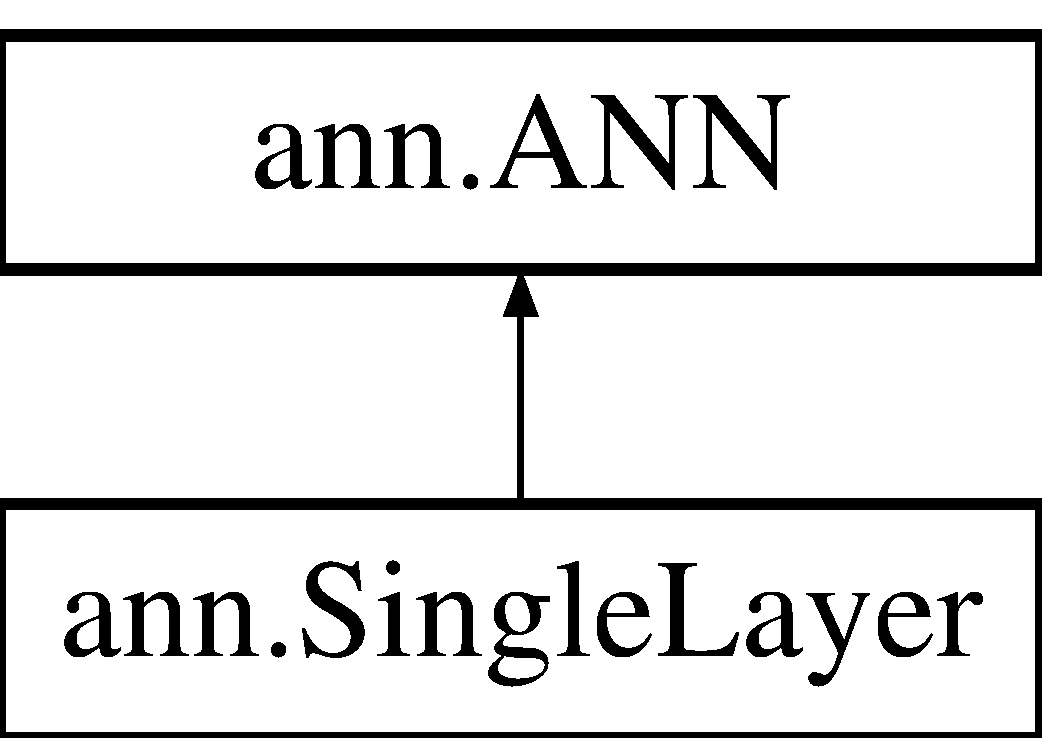
\includegraphics[height=2.000000cm]{classann_1_1_single_layer}
\end{center}
\end{figure}
\subsection*{Public Member Functions}
\begin{DoxyCompactItemize}
\item 
\mbox{\Hypertarget{classann_1_1_single_layer_ab973ce83e94cfcc1250ca95434950169}\label{classann_1_1_single_layer_ab973ce83e94cfcc1250ca95434950169}} 
{\bfseries Single\+Layer} (Map$<$ \hyperlink{classann_1_1_input}{Input}, \hyperlink{classann_1_1_output}{Output} $>$ training\+Data, Map$<$ \hyperlink{classann_1_1_input}{Input}, \hyperlink{classann_1_1_output}{Output} $>$ testing\+Data)
\item 
\mbox{\Hypertarget{classann_1_1_single_layer_abf681b102523232e632803dc563bdc07}\label{classann_1_1_single_layer_abf681b102523232e632803dc563bdc07}} 
\hyperlink{classann_1_1_output}{Output} {\bfseries feed} (\hyperlink{classann_1_1_input}{Input} in)
\item 
\mbox{\Hypertarget{classann_1_1_single_layer_ab03a33e2da33f038384dc51284b22f23}\label{classann_1_1_single_layer_ab03a33e2da33f038384dc51284b22f23}} 
Map$<$ Integer, Double $>$ {\bfseries train} (int nb\+Iterations)
\end{DoxyCompactItemize}


The documentation for this class was generated from the following file\+:\begin{DoxyCompactItemize}
\item 
C\+:/\+Users/\+Nick/\+Desktop/\+M1 M\+I\+A\+G\+E/\+Iam\+The\+One/\+Intelligence-\/\+Artificielle/\+Projet/src/ann/Single\+Layer.\+java\end{DoxyCompactItemize}

\hypertarget{classann_1_1_tanh}{}\section{ann.\+Tanh Class Reference}
\label{classann_1_1_tanh}\index{ann.\+Tanh@{ann.\+Tanh}}
Inheritance diagram for ann.\+Tanh\+:\begin{figure}[H]
\begin{center}
\leavevmode
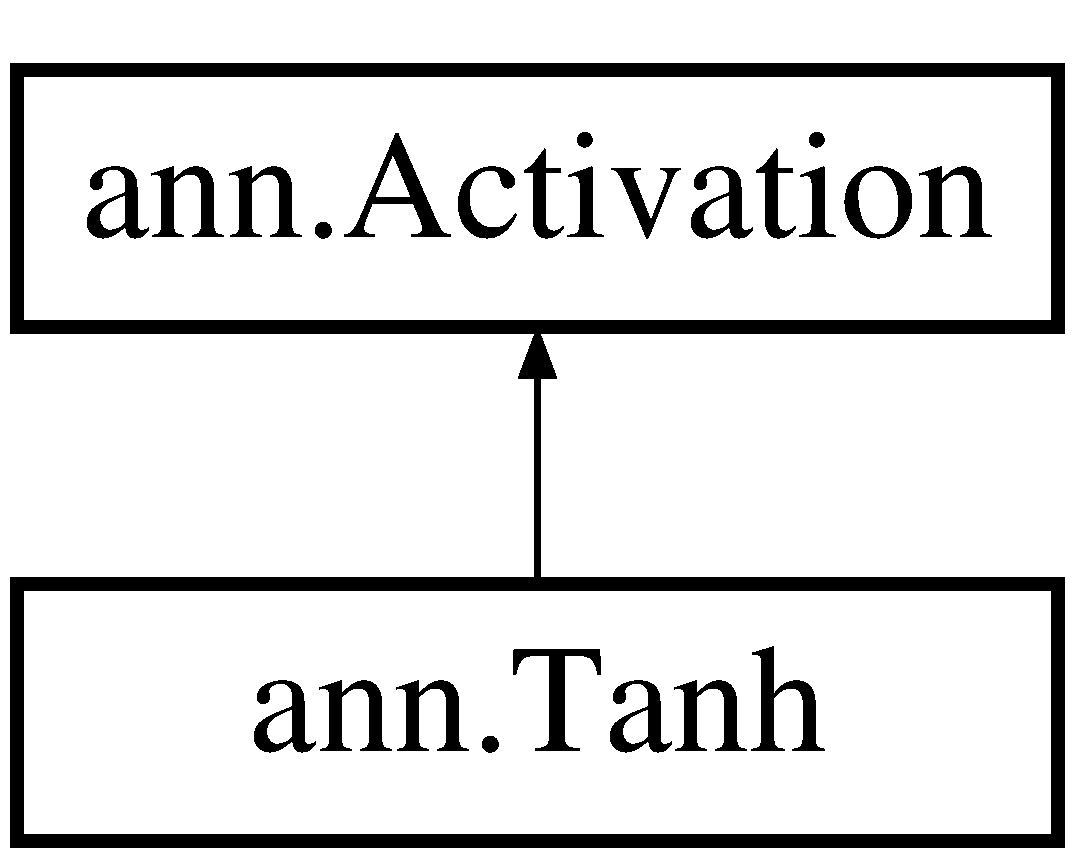
\includegraphics[height=2.000000cm]{classann_1_1_tanh}
\end{center}
\end{figure}
\subsection*{Public Member Functions}
\begin{DoxyCompactItemize}
\item 
\mbox{\Hypertarget{classann_1_1_tanh_a652b75e98b7ad29e16af82769df6b171}\label{classann_1_1_tanh_a652b75e98b7ad29e16af82769df6b171}} 
double {\bfseries activate} (double v)
\end{DoxyCompactItemize}


The documentation for this class was generated from the following file\+:\begin{DoxyCompactItemize}
\item 
C\+:/\+Users/\+Nick/\+Desktop/\+M1 M\+I\+A\+G\+E/\+Iam\+The\+One/\+Intelligence-\/\+Artificielle/\+Projet/src/ann/Tanh.\+java\end{DoxyCompactItemize}

%--- End generated contents ---

% Index
\backmatter
\newpage
\phantomsection
\clearemptydoublepage
\addcontentsline{toc}{chapter}{Index}
\printindex

\end{document}
